\documentclass{article}
\usepackage{amsmath}
\usepackage{dcolumn}
\usepackage{threeparttable}
\usepackage{geometry}
\usepackage{graphicx}
\graphicspath{{../figures/}} % Specify the relatlive path to the "images" folder

\newcolumntype{d}[1]{D{.}{.}{#1}}

% Placeholder paragraphs with text
\usepackage{blindtext}

% No indent for new paragraphs
\setlength\parindent{0pt}

% bibliography
\usepackage[
    backend=biber,
    style=bwl-FU,
    url=false,
    doi=false,
    eprint=false
]{biblatex}
\addbibresource{template-biblio.bib}

% ----------------------------------------------------------------------------

\usepackage{graphicx}  % for including images
\usepackage{titling}   % for more control over the title
\title{\textbf{Exploring the Relationship Between Bank Size And Sensitivity to Central Bank Policy Rate Changes}}

\author{Your Name}
\date{\today}

\begin{document}

\begin{titlepage}
    \centering
    \vspace*{-1.5cm} % Adjust the value as needed to reduce space
    \includegraphics[width=0.4\textwidth]{Test/University_of_Zurich_seal.svg.png} % Add your project logo
    
    \vspace{2cm}
    \Huge
    \textbf{Exploring the Relationship Between Bank Size And Sensitivity to Central Bank Policy Rate Changes}
    
    \vspace{1cm}
    \LARGE
    Subtitle or Project Description
    
    \vspace{1cm}
    \textbf{Authors:}\\ John Hojnacki \\ Matthew Aylward \\ Victoria Gemperle
    \vspace{1cm}
    
    \textbf{Date:}\\
    \thedate
    \vfill
    
\end{titlepage}


\section{Introduction}

    \linespread{1}  % Adjust the factor as needed
    
Central Banks around the world implement monetary policy in a variety of different ways, but one key transmission mechanism is typically a short-term rate at which commercial banks can borrow from the central bank. This rate, the ‘policy rate’, effectively becomes a floor on other rates, and measuring the sensitivity of other rates, such as the deposit rate, to changes in the policy rate, can give an indication as to how quickly monetary policy is transmitted in each cycle. For this project, the objective is to evaluate the sensitivity of deposit rates on consumer savings accounts to changes in the central banks’ policy rate across different economic cycles. The methodology can be expanded to evaluate multiple countries cross sectionally, or to evaluate a single country over several cycles.

\section{Data}

This project uses monthly policy rates and deposit rates for a particular country. If a country doesn't have a specific target, it may be extrapolated from a target range. In the example case, we use the midpoint of a range from the Swiss National Bank from 2000-2019, and then a target from 2019 onwards (they introduced a target at that time).\\

The methodology applied in this project is designed to be replicable across different countries and time periods, which allows for its usage in scenarios where central banks provide explicit targets, target ranges, or operate without a clearly defined target. The project can be employed to analyze and compare the sensitivity of deposit rates on consumer savings accounts to changes in central banks’ policy rates across different economic and temporal contexts. This cross-country and cross-temporal applicability assures the project's utility in capturing variations in monetary policy transmission mechanisms globally.

\section{History in a Swiss Context}

In December of 1999, the Swiss National Bank (‘SNB’) announced its intention to steer money market rates through the mechanism of a target range, a departure from the previous policy of targeting money supply. This change also coincided with the decision to begin tightening monetary policy over the next year. (source: SNB Quarterly bulletin, December 1999). This hiking cycle is the first of four which appears in the period of our analysis for Switzerland (2000, 2004, 4Q05-, and 2022-present day). However, the short hiking cycle in 2004 will be left out of our discussion for two reasons. First, the commentary from the SNB itself in the Monetary Policy Report at the time noted that while it was increasing the target range, overall policy remained expansionary. The second reason is that the hikes in this period were simply a reversal of the cuts which had taken place in March of 2003 to address deflation concerns. This resulted in no change in deposit rates, which interestingly had also experienced a muted reaction to the prior cut. The next true tightening of financial conditions began in March of 2006, and continued steadily until the Global Financial Crisis (“GFC”) necessitated easing of rates once again. The last hiking cycle begins in the wake of recovery from the Covid-19 Pandemic and continues through the time of this writing.  

\begin{figure}[h]
    \centering
    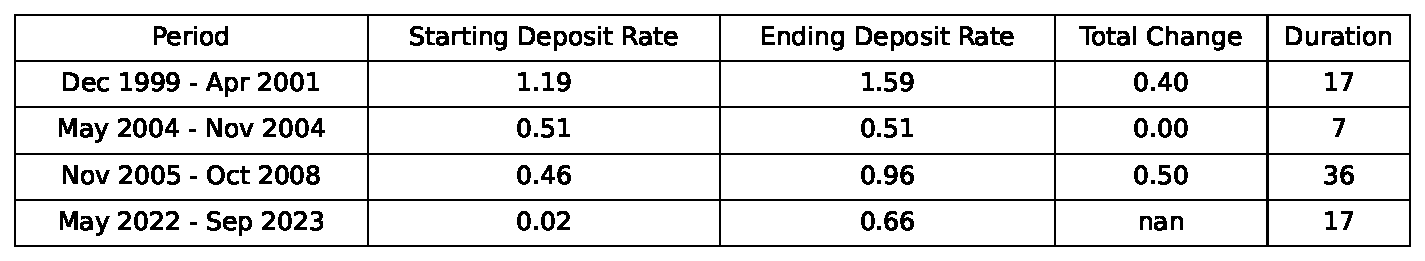
\includegraphics[width=0.8\textwidth]{Test/deposit_summary_SNB.pdf}
    \caption{Deposit Rates Summary across Hiking Periods}
    \label{fig:deposit_summary}
\end{figure}

\begin{figure}[h]
    \centering
    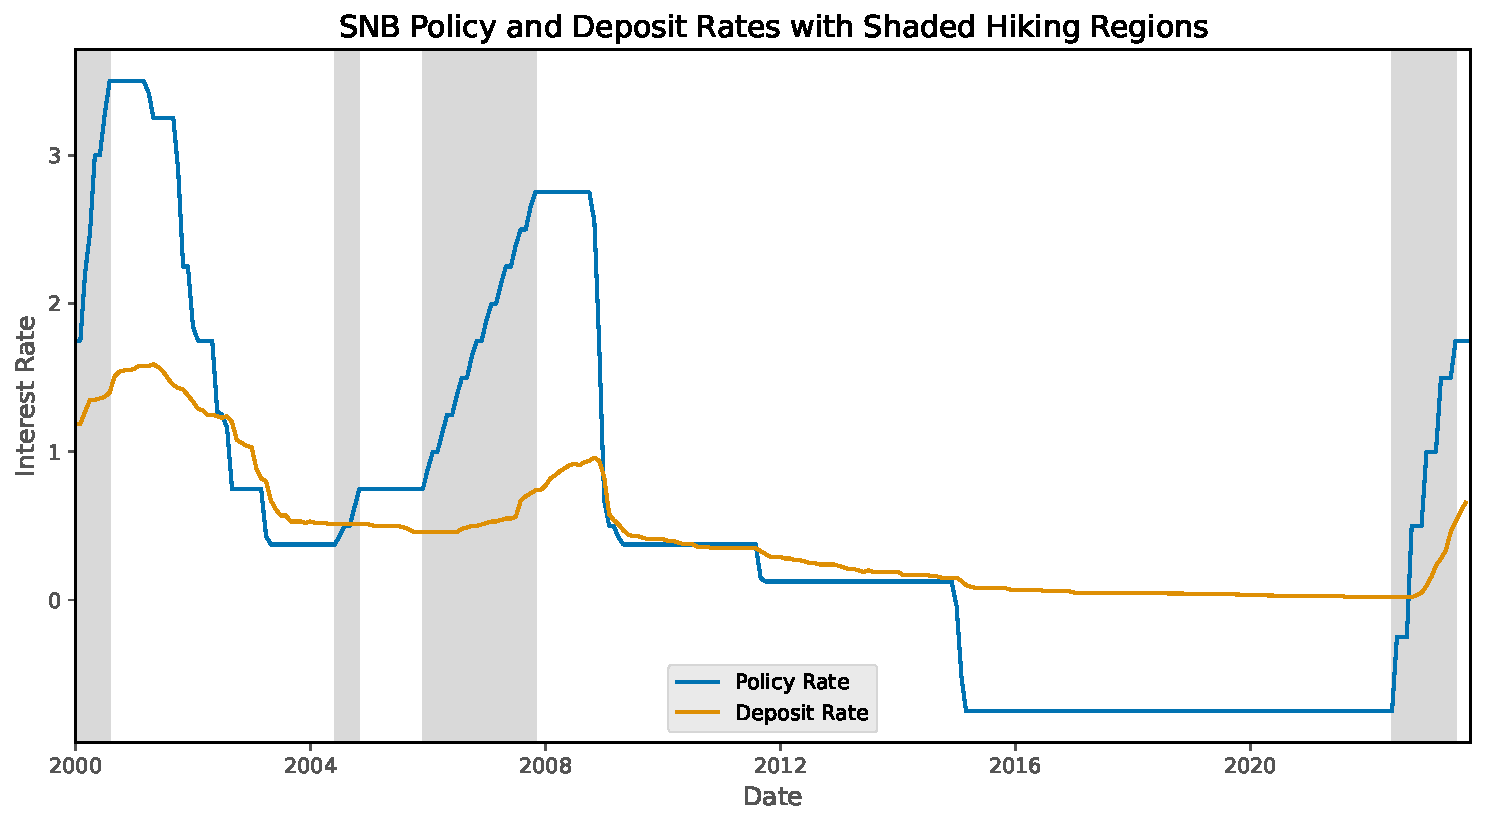
\includegraphics[width=0.8\textwidth]{Test/rates_shaded_SNB.pdf}
    \caption{Policy and Deposit Rates for Switzerland}
    \label{fig:rates_shaded}
\end{figure}

\begin{figure}[h]
    \centering
    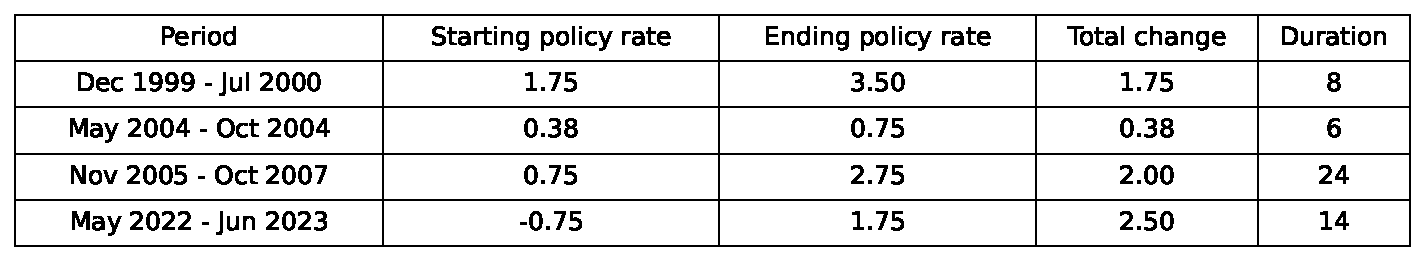
\includegraphics[width=0.8\textwidth]{Test/hiking_summary_SNB.pdf}
    \caption{Hiking Cycles Across Time}
    \label{fig:your_pdf}
\end{figure}

\begin{figure}[h]
    \centering
    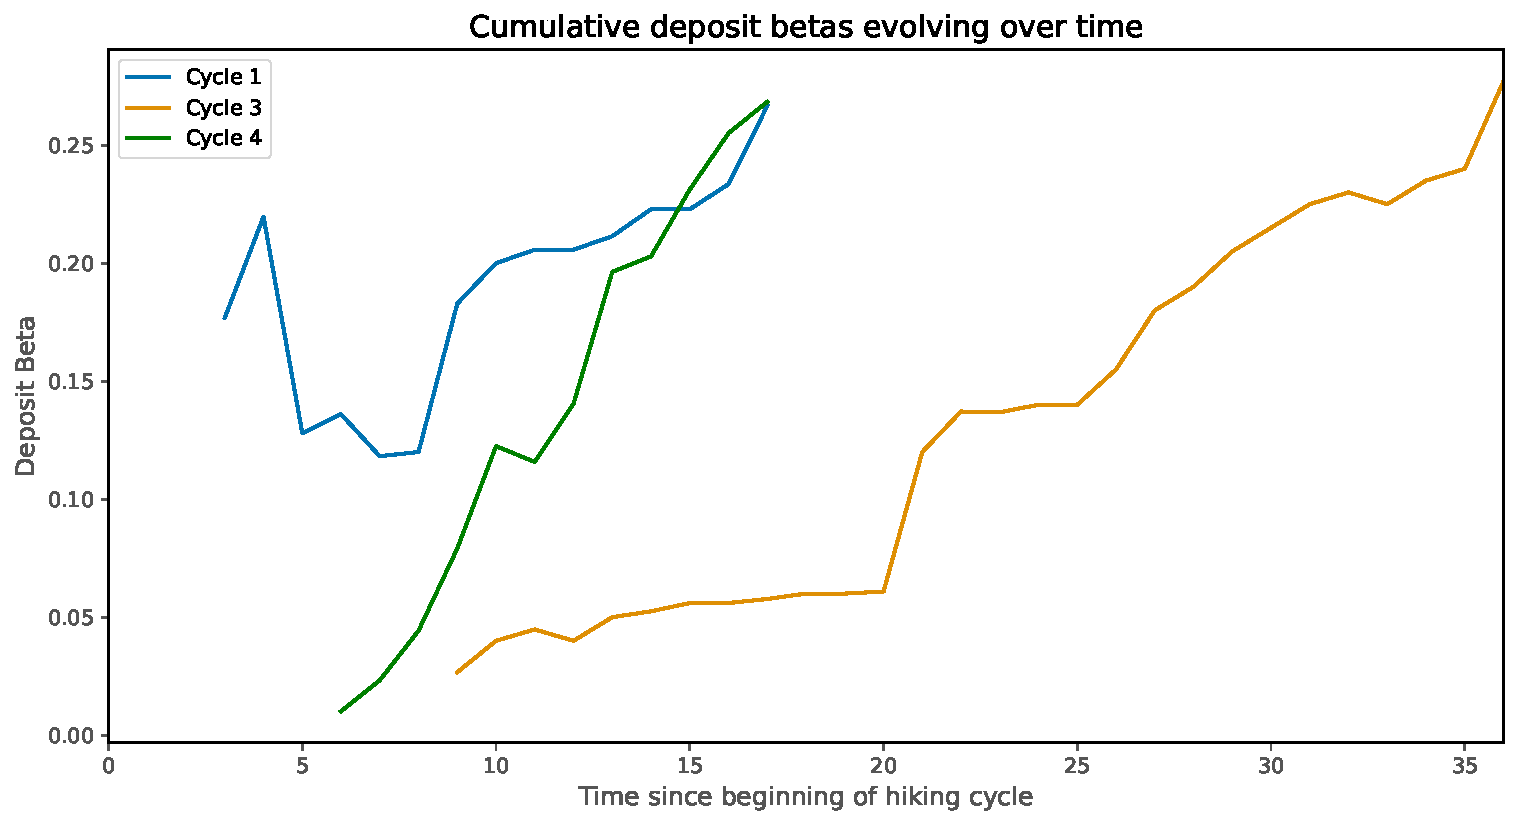
\includegraphics[width=0.8\textwidth]{Test/deposit_beta_SNB.pdf}
    \caption{Cumulative Swiss Deposit Betas in Hiking Cycles}
    \label{fig:your_pdf}
\end{figure}

% Bibliography section
\newpage  % Start a new page for the bibliography
\printbibliography[title={References}]  % "References" is the default title, you can customize it

\end{document}